\chapter[Resultados e Discussões]{Resultados}

\section{Solução Desenvolvida}

\subsection{Tecnologias e ferramentas utilizadas}

Para a construção da proposta de solução final foram utilizadas algumas ferramentas, tecnologias e bibliotecas ao longo do processo de desenvolvimento. A seguir estas estão elencadas junto com a motivação de sua utilização dentro da solução:

    \begin{quote}
    \begin{itemize}
        \item ReactJS: Biblioteca javascript utilizada para criar a interface dos diferentes módulos da solução.
        \item Material UI: Biblioteca de componentes ReactJS para um desenvolvimento ágil e fácil, sendo utilizado para criar um visual mais agradável para a aplicação.
        \item Web3.Js: Coleção de bibliotecas que possibilitam a interação com nós ethereum remotos, utilizando conexões HTTP ou ICP. Possibilitando assim que os clientes possam se comunicar com o contrato inteligente desenvolvido.
        \item Metamask: Extensão de navegador para acesso a aplicativos distribuídos(Dapps), onde a mesma injeta a API Ethereum do Web3 no contexto javascript dos sites. Também permite que os usuários criem e gerenciem suas próprias identidades e transações, trazendo uma interface segura para revisar transações antes de aceitá-las ou rejeitá-las.
        \item Docker e Docker-compose: Containers utilizados para facilitar o gerenciamento de dependências da aplicação assim como orquestrar facilmente os ambientes de desenvolvimento e produção das mesmas.
        \item TESTNET Ropsten (ETH): Rede ethereum que executa o mesmo protocolo que o Ethereum(main net) e é usada para fins de teste. O contrato inteligente da solução está registrado nesta e rede e todas as transações ocorrem em interações dentro dela.
        \item Ropsten Ethereum Faucet: Ferramenta utilizada para obter ethers gratuitos da rede de testes Ropstas para as contas utilizadas na solução;
        \item Digital Ocean: Serviço de hospedagem utilizado para hospedar os módulos(Dapps) desenvolvidos em um servidor, possibilitando que as aplicações possam ser acessadas sem a necessidade de executá-las localmente.
        \item Solidity: Linguagem de programação de alto nível por meio da qual é possível criar aplicações descentralizadas, em especial os smart contracts, na Ethereum. 
        \item Truffle: Um ambiente de desenvolvimento, framework de testes e pipeline de ativos para blockchains usando a Ethereum Virtual Machine (EVM). Tendo sido utilizado principalmente na fase inicial de construção do contrato inteligente, possibilitando o desenvolvimento do mesmo mais rapidamente.
        \item Ganache: Blockchain Ethereum pessoal utilizado executar testes, executar comandos e inspecionar o estado enquanto controla como a cadeia de blocos opera localmente.
    \end{itemize}
    \end{quote}
        
        
\subsection{Arquitetura da Solução}

A solução foi desenvolvida seguindo uma arquitetura cliente-servidor, representada na figura \ref{fig:dapp_arquitetura_solucao}. A parte do cliente nesta solução é composto pelas aplicações descentralizadas(Dapps) desenvolvidas, onde um módulo corresponde ao sistema utilizado pelas autoridades de trânsito e o outro módulo sendo o sistema de acesso dos motoristas. Já o servidor da solução corresponde a rede ethereum onde o \verb|deploy| do contrato inteligente foi feito e as transações são validadas pelos nós mineradores da rede, representado na figura \ref{fig:dapp_rede_ethereum}.

    \begin{figure}[h]
         \centering
         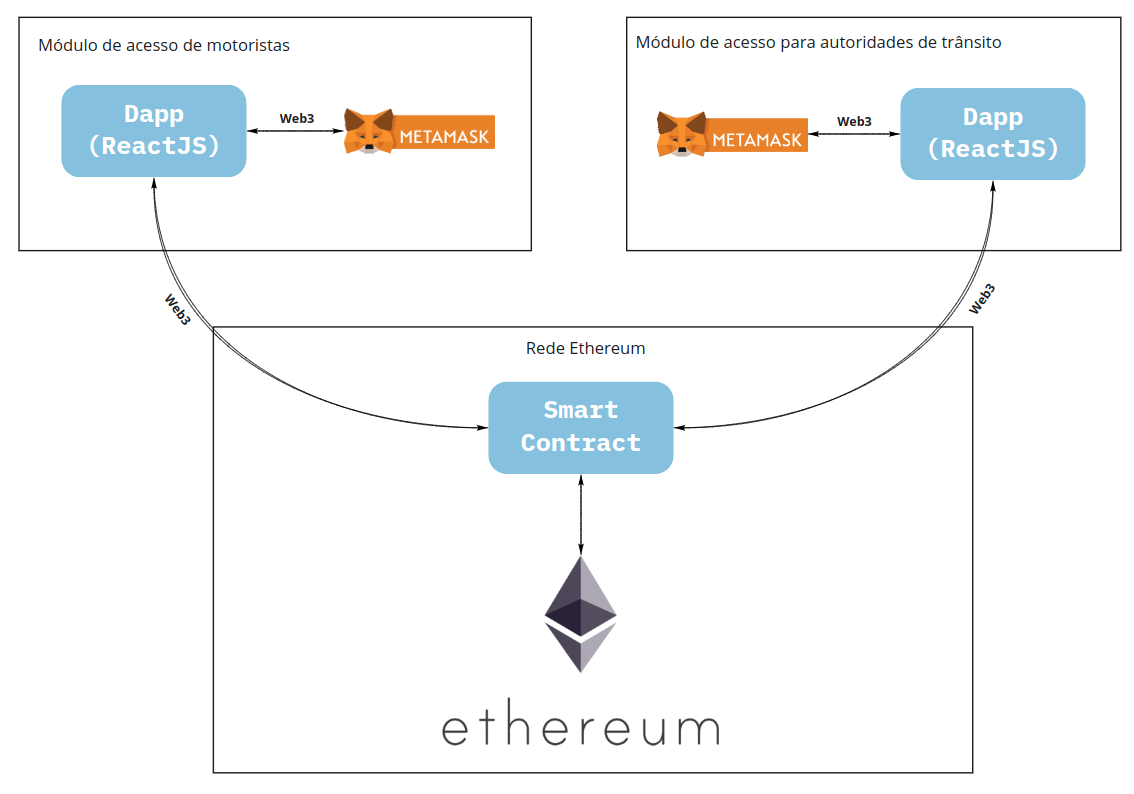
\includegraphics[scale=0.35]{figuras/capitulo_5/arquitetura_solucao.png}
         \caption{Representação da interação entre os módulos da solução - Imagem própria.}
         \label{fig:dapp_arquitetura_solucao}
    \end{figure}
                                                        
    \begin{figure}[h]
         \centering
         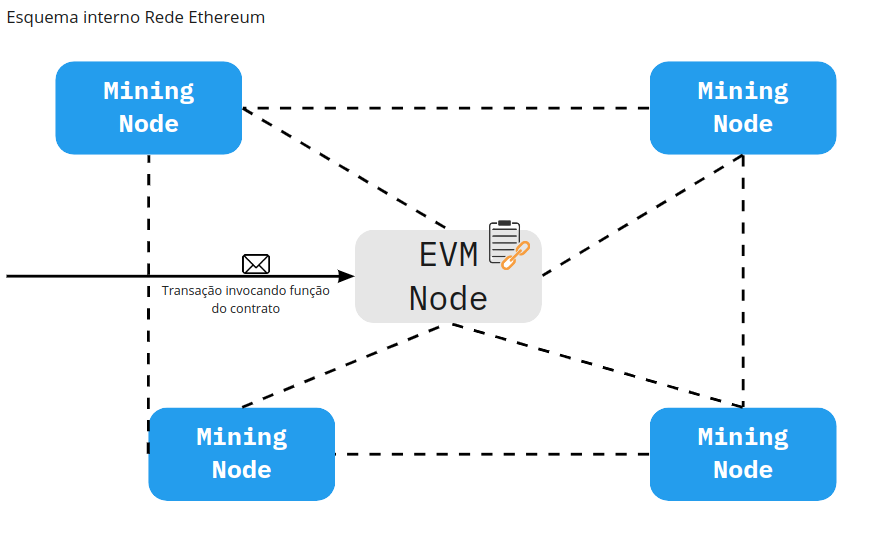
\includegraphics[scale=0.4]{figuras/capitulo_5/esquema_rede_ethereum.png}
         \caption{Representação da rede onde o contrato está na Ethereum Virtual Machine - Imagem própria.}
         \label{fig:dapp_rede_ethereum}
    \end{figure}
    
A rede ethereum atualmente utilizada para validar o protótipo e solução desenvolvida é a rede de testes ethereum Ropsten. A rede de testes Ropsten é executada utilizando os mesmos protocolos da rede principal Ethereum, porém sem custos financeiros atrelados a seu funcionamento podendo assim que testes sejam realizados sem a aquisição de Ethers. A rede provê por meio dos Faucets  a possibilidade dos usuários obterem Ethers de forma gratuita e poderem assim usufruir de todas as funcionalidades da rede como realizar transações, deploy de smart contracts, envio de ethers e etc.

\subsection{Módulos do Sistema}

A solução do sistema é composta por dois diferentes módulos, um para acesso do usuário motorista e outro para acesso das autoridades de trânsito. Cada módulo desse sistema corresponde a uma aplicação, sendo estas executadas de forma paralela.

As funcionalidades do sistema possuem especificidades de acordo com o perfil de usuário que está utilizando o sistema, o que demanda um nível de autenticação para acesso a estas informações. A proposta de trabalho traz algumas premissas, onde as premissas II e IV indicam que  usuário do sistema seja ele um motorista ou autoridade de trânsito possui uma conta e uma única chave de acesso que o representa. Para realizar a autenticação dentro dos módulos do sistema, estas premissas são utilizadas como base e ocorre utilizando-se esta chave única.

\subsection{Autenticação dos usuários nos módulos sistema}

A autenticação nas aplicações não ocorre por meio de login e senha como usualmente em sistemas, onde nesta solução a autenticação é feita com o auxílio da extensão metamask. Optou-se por esta abordagem para que o usuário tenha suas informações ainda mais resguardadas sem a necessidade de armazená-las em um local externo, garantindo assim que o princípio confidencialidade da segurança computacional definido por Stallings esteja presente em meio as aplicações.

O fluxo de autenticação ocorre da seguinte maneira em meio as aplicações:

    \begin{quote}
        \begin{enumerate}
            \item Quando o usuário requisita acesso a uma página do sistema, conta ativa no momento na extensão metamask é obtida com auxílio da extensão Web3;
            \item É feita uma chamada de função ao smart contract onde é verificado se esta conta existe em meio aos arrays de motorista ou autoridades de trânsito de acordo com o módulo acessado;
            \item Se a conta está presente no array solicitado a página é renderizada e o usuário está assim autorizado no sistema. No caso de negativa desta condição o usuário não é autorizado e não consegue acessar as funcionalidades do sistema.
        \end{enumerate}
    \end{quote}

\subsection{Autorização dentro do smart contract}

Na aplicação possuímos um esquema de autenticação de forma a garantir que somente pessoas autorizadas possuam acesso a determinadas funcionalidades, porém como garantir que isso também ocorra dentro do smart contract que é público dentro da rede?

Dentro da rede Ethereum caso uma pessoa tenha o endereço do contrato o mesmo poderá visualizar todas as transações realizadas, assim como realizar chamadas de funções declaradas como públicas no código fonte.

Como todas as contas as podem chamar as funções presente no contrato é feito mais um nível de autenticação dentro de cada função, onde caso a autenticação falhe a execução da função é interrompido. Este controle é feito utilizando a função \textit{require()} presente na linguagem solidity, onde é verificado se o address da conta \textit{sender} está registrado e autorizado a realizar este procedimento.

\subsection{Funcionalidades}

A proposta de solução elencou na seção \ref{section:funcionalidades_propostas} algumas funcionalidades a serem desenvolvidas de forma a solucionar o problema levantado no desenvolvimento deste trabalho. A solução desenvolvida conseguiu contemplar todas estas funcionalidades propostas e consideradas fundamentais para o funcionamento do sistema RENAINF, demonstrando a possibilidade de adaptação de um sistema existente utilizando-se a tecnologia blockchain.

Porém tornou-se necessário uma adaptação na funcionalidade de Recurso/Cancelamento de infração de trânsito proposta inicialmente. Ao se mapear os requisitos de forma que essa atenda ao RENAINF e o CTB, ocorreu um erro de interpretação onde a proposta trazia inicialmente que a autoridade de trânsito que realizou o registro da infração seria também responsável por julgar este recurso e isto acaba não seguindo totalmente o processo adotado no código CTB. O Artigo 287 do CTB diz que uma junta de trânsito (Jari) será responsável pelo julgamento do recurso proposto e não a autoridade que registrou a infração, então foi necessário esta adaptação nos requisitos iniciais.

Para o funcionamento desta funcionalidade na solução atual a Jari é considerada uma autoridade de trânsito, que só possui acesso a essa funcionalidade, e é única em todo o sistema. Onde atualmente todos os recursos realizados pelos motoristas são direcionados a essa única Jari registrada previamente na criação do contrato, atendendo assim o que está registrado no CTB e corrigindo o requisito errôneo mapeado anteriormente.

